\documentclass[tikz,border=10pt]{standalone}
\usepackage{amsmath}
\usepackage{amssymb}
\usepackage{tikz}
\usetikzlibrary{arrows.meta,calc}

\definecolor{figazul}{RGB}{2,132,199}
\definecolor{figrojo}{RGB}{220,38,38}
\definecolor{figverde}{RGB}{22,163,74}
\definecolor{figmorado}{RGB}{124,58,237}

\begin{document}
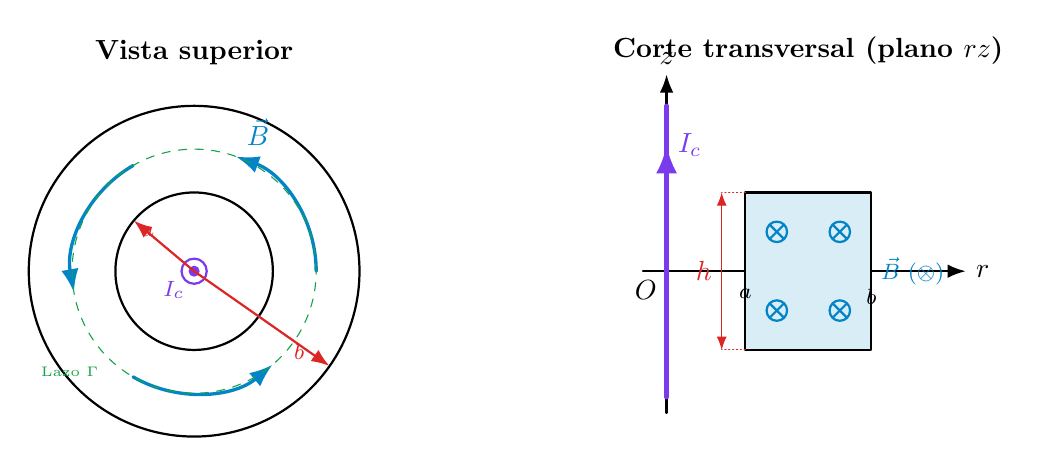
\begin{tikzpicture}[>=Latex, line cap=round, line join=round]
  % -------------------------------------------------------------
  % Panel Izquierdo: Vista superior (plano r-phi)
  % -------------------------------------------------------------
  \begin{scope}[xshift=0cm]
    \node[above, font=\bfseries] at (0, 2.5) {Vista superior};

    % Círculos concéntricos de radios a = 1.0 y b = 2.1
    \draw[thick] (0,0) circle (2.1);
    \draw[thick] (0,0) circle (1.0);

    % Centro con cable axial Ic (morado)
    \fill[color=figmorado] (0,0) circle (2pt);
    \draw[thick, color=figmorado] (0,0) circle (0.16);
    \fill[color=figmorado] (0,0) circle (0.05);
    \node[below left, font=\footnotesize, color=figmorado] at (0,0) {$I_c$};

    % Líneas de campo B azimutales en sentido antihorario (+phi)
    \draw[->, very thick, color=figazul] (0:1.55) arc (0:70:1.55) node[above right, color=figazul] {$\vec{B}$};
    \draw[->, very thick, color=figazul] (120:1.55) arc (120:190:1.55);
    \draw[->, very thick, color=figazul] (240:1.55) arc (240:310:1.55);

    % Cotas de radio
    \draw[->, thick, color=figrojo] (0,0) -- (140:1.0);
    \node[above left, color=figrojo, font=\footnotesize] at (140:0.5) {$a$};

    \draw[->, thick, color=figrojo] (0,0) -- (-35:2.1);
    \node[below right, color=figrojo, font=\footnotesize] at (-35:1.4) {$b$};

    % Lazo amperiano opcional
    \draw[dashed, thin, color=figverde] (0,0) circle (1.55);
    \node[below left, font=\tiny, color=figverde] at (225:1.55) {Lazo $\Gamma$};
  \end{scope}

  % -------------------------------------------------------------
  % Panel Derecho: Corte transversal (plano rz)
  % -------------------------------------------------------------
  \begin{scope}[xshift=6.0cm]
    \node[above, font=\bfseries] at (1.8, 2.5) {Corte transversal (plano $rz$)};

    % Ejes r y z
    \draw[->, thick] (-0.3,0) -- (3.8,0) node[right] {$r$};
    \draw[->, thick] (0,-1.8) -- (0,2.5) node[above] {$z$};
    \node[below left] at (0,0) {$O$};

    % Cable central en r = 0 a lo largo de z (morado)
    \draw[ultra thick, color=figmorado] (0, -1.6) -- (0, 2.1);
    \draw[->, ultra thick, color=figmorado] (0, 0.8) -- (0, 1.6) node[right, color=figmorado] {$I_c$};

    % Sección transversal rectangular entre r = a (1.0) y r = b (2.6), altura h (2.0)
    % De z = -1.0 a z = 1.0
    \draw[thick, fill=figazul!15] (1.0, -1.0) rectangle (2.6, 1.0);

    % Símbolos de campo entrante B (otimes) en grilla regular 2x3
    \foreach \x in {1.4, 2.2} {
      \foreach \y in {-0.5, 0.5} {
        \draw[thick, color=figazul] (\x,\y) circle (0.13);
        \draw[thick, color=figazul] (\x-0.09,\y-0.09) -- (\x+0.09,\y+0.09);
        \draw[thick, color=figazul] (\x-0.09,\y+0.09) -- (\x+0.09,\y-0.09);
      }
    }
    \node[right, font=\footnotesize, color=figazul] at (2.6, 0) {$\vec{B}$ ($\otimes$)};

    % Cotas de radio a y b en el eje r
    \draw[line width=0.8pt] (1.0, 0.1) -- (1.0, -0.1) node[below, font=\footnotesize] {$a$};
    \draw[line width=0.8pt] (2.6, 0.1) -- (2.6, -0.1) node[below, font=\footnotesize] {$b$};

    % Cota de altura h
    \draw[<->, thin, color=figrojo] (0.7, -1.0) -- (0.7, 1.0) node[midway, left, color=figrojo] {$h$};
    \draw[densely dotted, thin, color=figrojo] (1.0, -1.0) -- (0.7, -1.0);
    \draw[densely dotted, thin, color=figrojo] (1.0, 1.0) -- (0.7, 1.0);
  \end{scope}
\end{tikzpicture}
\end{document}
